\documentclass[varwidth]{standalone}

\usepackage{tikz}
\usetikzlibrary{shapes.geometric, arrows, calc, positioning}

\tikzstyle{morning} = [rectangle, rounded corners, minimum width=3cm, minimum
height=2cm,text centered, text width = 3cm, draw=black, fill=green!30]

\tikzstyle{afternoon} = [rectangle, rounded corners, minimum width=3cm, minimum
height=2cm,text centered, text width = 3cm, draw=black, fill=red!30]

\tikzstyle{evening} = [rectangle, rounded corners, minimum width=3cm, minimum
height=2cm,text centered, text width = 3cm, draw=black, fill=blue!30]


\tikzstyle{arrow} = [thick,->,>=stealth]

\usepackage{graphicx}


\title{Timetable(Version 2)}
\author{Qiyuan Pu}

\begin{document}
\maketitle{}


\includegraphics[height=3em]{writing.png}

\includegraphics[height=3em]{graduation.png}

\begin{figure}
  \centering


    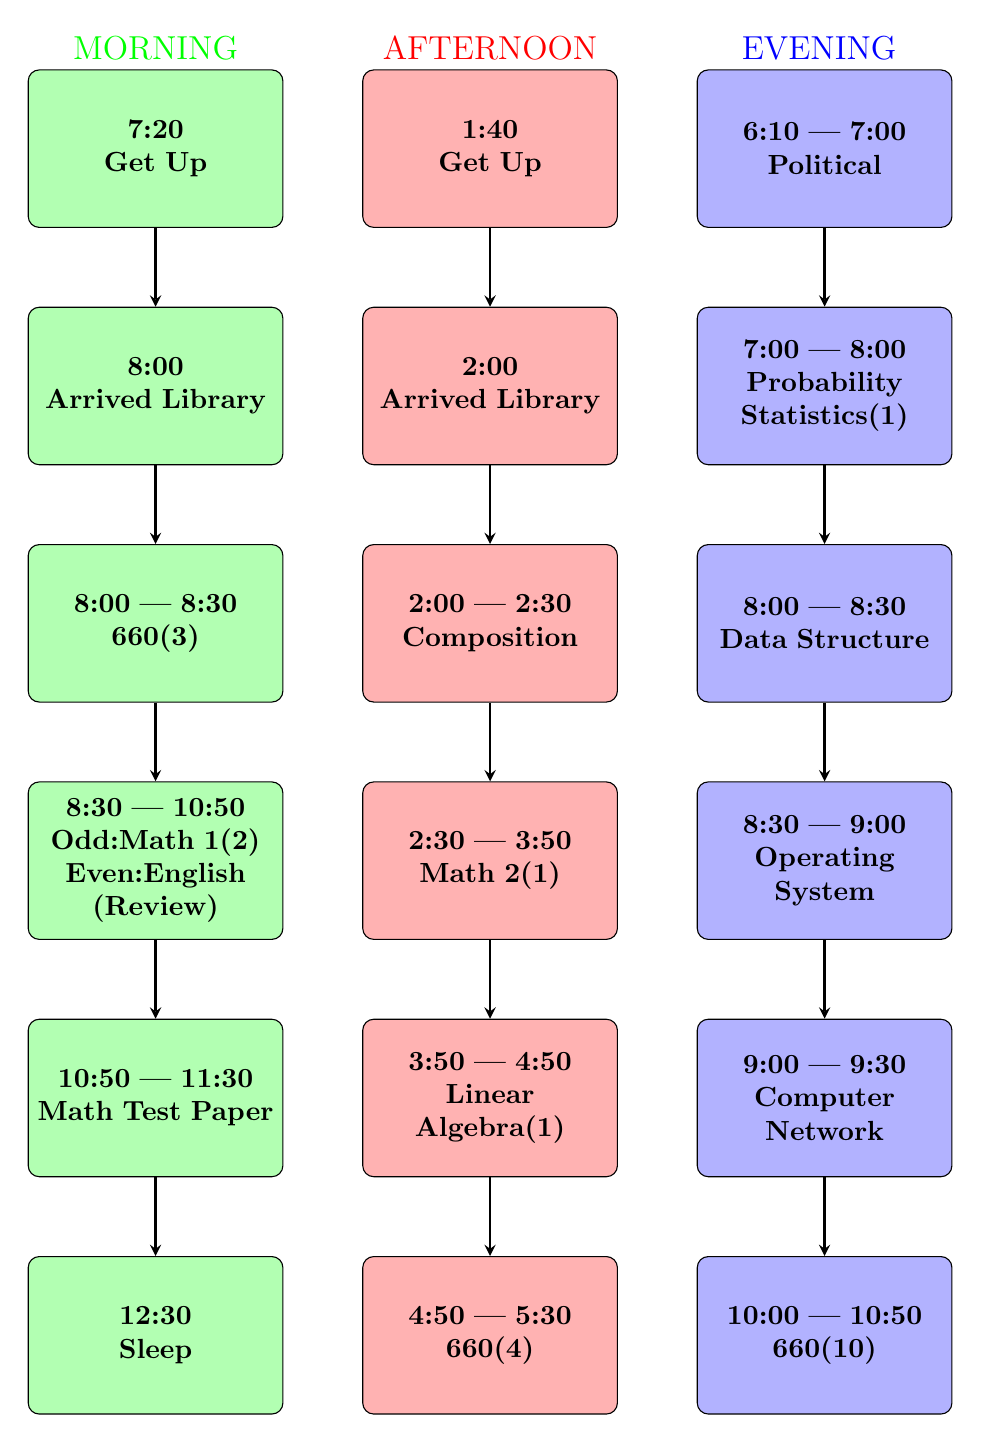
\begin{tikzpicture}
      \node (mor2) [morning, label=above: {\large \color{green} MORNING}] {\bf 7:20 \\ Get Up};
      \node (mor3) [morning, below=of mor2] {\bf 8:00 \\ Arrived Library};
      \node (add1) [morning, below=of mor3] {\bf 8:00 — 8:30 \\ 660(3)};
      \node (mor4) [morning, below=of add1] {\bf 8:30 — 10:50 Odd:Math 1(2) Even:English \\ (Review)};
      \node (mor5) [morning, below=of mor4] {\bf 10:50 — 11:30 \\ Math Test Paper};
      \node (mor6) [morning, below=of mor5] {\bf 12:30 \\ Sleep};

      \node (aft2) [afternoon, right=of mor2, label=above: {\large \color{red} AFTERNOON}] {\bf 1:40 \\ Get Up};
      \node (aft3) [afternoon, below=of aft2] {\bf 2:00 \\ Arrived Library};
      \node (add2) [afternoon, below=of aft3] {\bf 2:00 — 2:30 \\ Composition};
      \node (aft4) [afternoon, below=of add2] {\bf 2:30 — 3:50 \\ Math 2(1)};
      \node (aft5) [afternoon, below=of aft4] {\bf 3:50 — 4:50 \\ Linear \\ Algebra(1)};
      \node (aft6) [afternoon, below=of aft5] {\bf 4:50 — 5:30 \\ 660(4)};

      \node (eve1) [evening, right=of aft2, label=above: {\large \color{blue} EVENING }] {\bf 6:10 — 7:00 \\ Political};
      \node (eve2) [evening, below=of eve1] {\bf 7:00 — 8:00 \\ Probability Statistics(1)};
      \node (eve3) [evening, below=of eve2] {\bf 8:00 — 8:30 \\ Data Structure};
      \node (eve4) [evening, below=of eve3] {\bf 8:30 — 9:00 \\ Operating System};
      \node (add3) [evening, below=of eve4] {\bf 9:00 — 9:30 \\ Computer Network};
      \node (eve5) [evening, below=of add3] {\bf 10:00 — 10:50 \\ 660(10)};

      \draw [arrow] (add1) -- (mor4);
      \draw [arrow] (eve4) -- (add3);
      \draw [arrow] (add3) -- (eve5);
      \draw [arrow] (eve3) -- (eve4);
      \draw [arrow] (eve2) -- (eve3);
      \draw [arrow] (eve1) -- (eve2);
      \draw [arrow] (mor3) -- (add1);
      \draw [arrow] (mor4) -- (mor5);
      \draw [arrow] (mor5) -- (mor6);
      \draw [arrow] (mor2) -- (mor3);
      \draw [arrow] (aft2) -- (aft3);
      \draw [arrow] (aft3) -- (add2);
      \draw [arrow] (aft4) -- (aft5);
      \draw [arrow] (aft5) -- (aft6);
      \draw [arrow] (add2) -- (aft4);
    \end{tikzpicture}
  

  % \textcolor{red}{Fighting}

\end{figure}

\includegraphics[height=3em]{trophy.png}
\dotfill

\includegraphics[height=3em]{biking.png}

% \textcolor{red}{Fighting}

\end{document}



%%% Local Variables:
%%% mode: latex
%%% TeX-master: t
%%% End:
